\chapter{Evaluation}
\label{chap:evaluation}
% "Moreover, under large record size (e.g., 1KB and above), B+ tree tend to have smaller write amplification than LSM-tree." - from "Closing the B+-Tree vs. LSM-Tree Write Amplification Gap on Modern Storage Hardware with Built-in Transparent Compression", Qiao et al., FAST 2022
% Good evaluation paper: https://dl.acm.org/doi/pdf/10.1145/3183713.3196895
% To adhere to the DAM model, can't we assume that all inner nodes are cached in memory, but leafs are not? see "A Comparison of Fractal Trees to Log-Structured Merge (LSM) Trees"

% Observations:
% We erase a lot of entries in the Delta Tree, which causes a lot of fragmentation and caused significantly more nodes.
% - The higher the fanout of the tree, the higher the write amplification we introduce in the Delta Tree itself.
% - We essentially amplified the write amplification in the system.
% WA becomes worse the bigger the Delta Tree becomes in relation to the Base Tree.
% - When we compacitified after every erase, we saw a reduction in write amplification again.
% - Now we reduce write amplification for small threshold (5-10%), but increase it for higher thresholds (20-50%).

% - We reduce write amplification only if we write out a Delta Tree node with more than one entry since the last write-out.
% - If we always write out a Delta Tree node already after a single change, we do not benefit.
% - We should see that effect when our buffer is too small and we cannot cache anything.
% - Buffering only makes sense if we can cache changes.

% - Everytime we load a B-Tree node, we perform a lookup into the Delta Tree.

% Mention that we do not take into accound construction and destruction of the index, since we are interested in steady state performance.

\section{Experimental Setup}
Since we are interested in write amplification, we observe the number of page writes to disk for different workloads and different memory limitations.
This way, our results are not biased by the specific implementation, optimizations, and hardware that we run our experiments on.
All experiments were conducted locally on a Apple MacBook Pro with the specification listed in \autoref{tab:hardware-specs}.

\begin{table}[htbp]
\centering
\caption{Hardware Specifications}
\label{tab:hardware-specs}
\begin{tabular}{ll}
\toprule
\textbf{Component} & \textbf{Specification} \\ 
\midrule
Device & Apple MacBook Pro (2021) \\
Processor (CPU) & Apple M1 Pro (8-core, up to 3.2\,GHz) \\
GPU & Integrated 14-core Apple GPU \\
Memory (RAM) & 16\,GB \\
Storage & 512\,GB NVMe SSD \\
Operating System & macOS Sonoma 14.6.1 \\
\bottomrule
\end{tabular}
\end{table}

\section{Workloads and Datasets}
We evaluate our approach on synthetic and real-world datasets.
The real-world dataset allows us to evaluate our approach on realistic data distributions and access patterns.
With the synthetic dataset, we can control the data distribution to evaluate the performance of our approach under different scenarios.
This allows us to identify the strengths and weaknesses of our approach.

We will be evaluating our system as a whole, benchmarking the database with the different indices to gain a holistic view of the performance.
To take a closer look at the indices themselves, we will also be benchmarking the indices in isolation, without the overhead of the database system.
For example, when benchmarking the whole database, we have to maintain the table data as well as the index, which introduces additional overhead.
When benchmarking the index in isolation, we can focus on the performance of the index itself.

\subsection*{Wikipedia Pageviews Workload}
We use an augmented Wikipedia Pageviews dataset \cite{wiki_pageviews} as a real-world dataset for our evaluation.
The primary goal of this dataset is to evaluate the performance of our approach on realistic data distributions and access patterns.
The dataset contains pageview statistics for all Wikipedia articles within a certain time frame.
It is publicly available and can be downloaded from the Wikimedia Dumps website\footnote{https://dumps.wikimedia.org/other/pageviews/}.
Each pageview record is of the form 
$$
\texttt{en Google\_Chrome 10406 0}
$$
consisting of the domain code, the page title, the number of views, and  the total response size in bytes.

\subsubsection*{Data Augmentation}
We use the hourly Pageview Wikipedia dataset from 1st of October 2025 at 00:00 UTC as our base dataset.
We augment the dataset in the following way:
\begin{enumerate}
    \item We filter out all non-English articles, i.e., we only keep articles with the domain code \texttt{en}.
    \item For benchmarks with integer keys, we turn the page title into an integer key. For benchmarks with variable-sized keys, we use the original page title as key.
    \item We create a lookup operation for each view of an article, i.e., if an article has 100 views, we create 100 lookups for that article.
    % TODO: update the actual percentage we used.
    \item To generate a mixed workload, we turn a 5\% percentage of the lookups into updates. This assumes that an article with more views is more likely to be updated.
    \item We then shuffle the operations to create a mixed workload.
    % TODO: update the percentage of the sample we used.
    \item To create a smaller dataset, we take a random 5\% sample of the articles.
\end{enumerate}

To populate the database, we insert all articles from filtered dataset once.
We then run the workload on the database or on the indices directly.

\subsubsection*{Workload Characteristics}
\label{sec:workload-characteristics}
The resulting workload has the following characteristics:
\begin{itemize}
    \item The dataset contains 59,240 distinct articles, translating to 59,240 distinct keys in the database.
    \item The workload contains 146,068 lookup operations in total, of which 7,303 were turned into updates (\textasciitilde5\%).
    \item The keys follow a Zipf-like distribution, i.e. a small number articles are very popular and receive a large number of operations, while the majority of articles receive only a few. 
    \item In fact, 40,670 articles (\textasciitilde69\%) are viewed only once in the dataset. 
    The most viewed article, \textit{Jon\_Stewart}, received 2,998 views (\textasciitilde10\% of all views).
    \item Overall, we update 5,724 distinct articles (\textasciitilde10\% of all articles) in the generated workload, whereas the majority of articles (\textasciitilde86\%) are only updated once.
    The most frequently updated article, \textit{Jon\_Stewart}, is updated 132 times (\textasciitilde10\% of all updates).
    \item The keys are variable-sized strings with an average length of 20.5 characters, a maximum length of 236 characters and a minimum length of 1 character.
\end{itemize}

% \subsection*{Synthetic Data}
% TODO

\section{Results and Analysis}
In this section, we present the results of our benchmark experiments and analyze the performance of the B-Tree and BBB-Tree indices.
Our primary metric for this evaluation is the number of page writes to disk, which directly correlates to the write amplification of the index.

% 4. Then, consider different update ratios (0\%, 5\%, 20\%, 50\%).
% 5. Then, consider different workloads (only inserts, only lookups).


The goal of this evaluation is to determine whether the BBB-Tree can reduce page writes compared to a traditional B-Tree under different workloads and memory constraints.
Additionally, we want to understand the trade-offs involved in using a BBB-Tree.

\subsection*{Write Amplification}
For a first analysis, we consider the write amplification of the B-Tree and BBB-Tree indices when running the mixed Wikipedia Pageviews workload on the database.
We run the workload with 4 KB pages, a buffer pool of 500 pages, and a write threshold of 5\% (i.e. we only write pages to disk if at least 5\% of the page has been modified in the case of a BBB-Tree index).
We compare the number of page writes to disk for both indices.
To gain a holistic view of the performance, we run the workload on the database as well as on the indices directly.
The results are shown in \autoref{fig:both}.
When running the workload on the database as a whole (\autoref{fig:sub1}), we see a reduction in page writes of \textasciitilde23\% when using the BBB-Tree compared to the B-Tree.
When running the workload on the indices directly (\autoref{fig:sub2}), we see a more significant reduction in page writes of \textasciitilde66\% when using the BBB-Tree compared to the B-Tree.

There are two main reasons for the difference in write amplification reduction between the two scenarios.
\begin{enumerate}
  \item \textbf{Relative Impact}: Firstly and more obviously, when running the workload on the database, we have more pages in the system that are not affected by our method.
Our method effects a smaller fraction of the total number of pages in the buffer, therefore our relative impact is naturally smaller.
When running the workload on the indices directly, we can focus on the performance of the method itself without the overhead of maintaining the table data.
Therefore, we will focus on the results when running the workload on the indices in isolation in the following analysis.
  \item \textbf{Memory Constraints}: More importantly, the indices have different memory constraints in the two scenarios.
When running the workload on the database, the indices have to share the buffer pool with the table data.
When running isolated, the indices can use the full memory available in the system. 
In the metrics collected during the benchmark runs (\autoref{tab:bm_pageviews_mixed_combined}), we can see that we have 10-15\% higher buffer hit rates when running the workload on the indices directly.
While both indices have the same memory available and higher buffer hit rates when running isolated, the BBB-Tree performs better in terms of write amplification reduction.
\end{enumerate}

These findings indicate that the BBB-Tree can significantly reduce write amplification compared to a traditional B-Tree, especially when the index can effectively utilize the available memory.
To investigate this further, we will run the workload under different memory constraints in the following section.

\begin{figure}[htbp]
  \centering
  \begin{subfigure}[b]{0.49\textwidth}
    \centering
    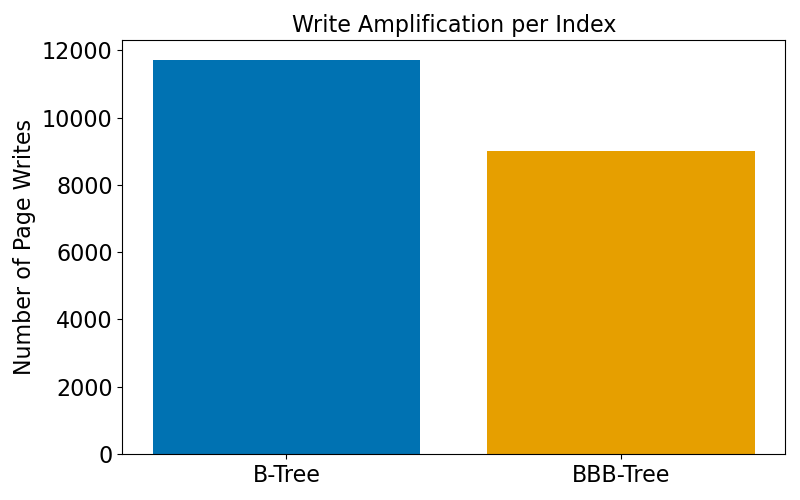
\includegraphics[width=\textwidth]{figures/evaluation/pageviews_mixed_db.png}
    \caption{Running the workload on the database with different indices.}
    \label{fig:sub1}
  \end{subfigure}
  \hfill
  \begin{subfigure}[b]{0.49\textwidth}
    \centering
    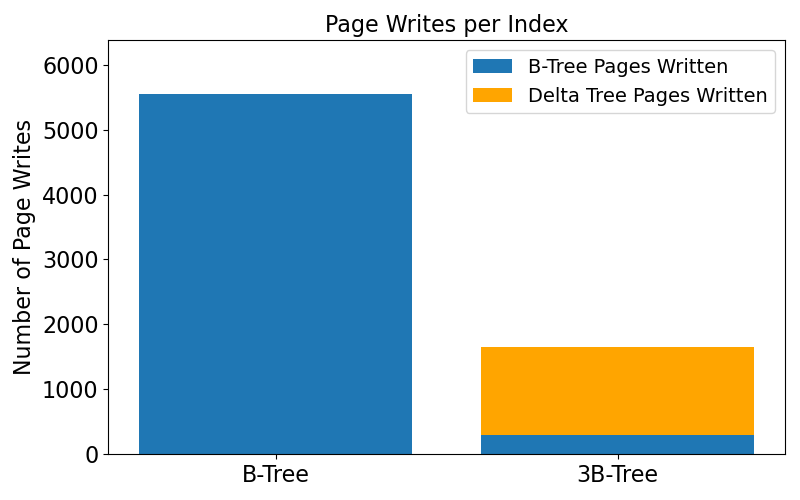
\includegraphics[width=\textwidth]{figures/evaluation/pageviews_mixed_index.png}
    \caption{Running the workload on the indices directly.}
    \label{fig:sub2}
  \end{subfigure}
  \caption{Running the mixed Wikipedia Pageviews workload with 5\% updates, 4 KB pages, a buffer pool of 500 pages, and a write threshold of 5\%. We see a significant difference in write amplification reduction when running the index as part of the database vs. running it in isolation.}
  \label{fig:both}
\end{figure}

\subsection*{Impact of Memory Constraints}
To understand the impact of memory constraints on the performance of the BBB-Tree, we run the same workload with different buffer pool sizes.
The workload produces a B-Tree of 606 nodes in total. We vary the buffer pool size from 50 to 700 pages, while keeping the page size at 4 KB.
The results are shown in \autoref{fig:buffer_sizes}.

\begin{figure}[htbp]
  \centering
  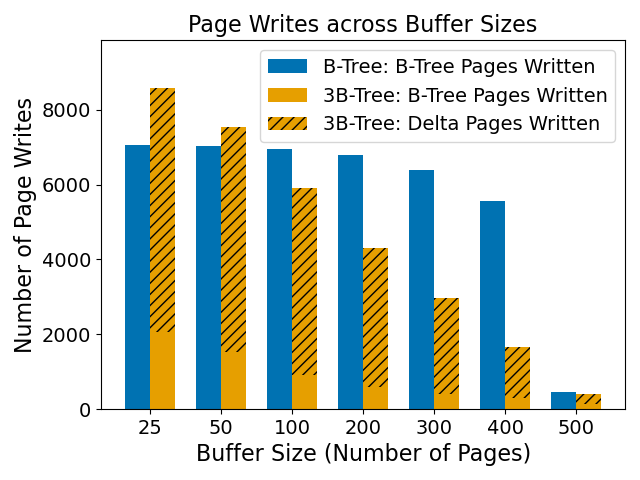
\includegraphics[width=0.7\textwidth]{figures/evaluation/pageviews_buffer_sizes.png}
  \caption{The impact of buffer pool size on the amount of page writes per index with a 4 KB page size and a 5\% write threshold. The BBB-Tree performs better with higher buffer pool sizes, as it can accumulate more changes in memory before writing them to disk. When the buffer fits the whole index, we perform no page writes at all.}
  \label{fig:buffer_sizes}
\end{figure}

\inlinesection{Low Memory Capacity.}
With a buffer pool of 50 to 100 pages, we have little memory to cache changes.
The BBB-Tree suffers from the limited memory more than the B-Tree and we even see an increase in page writes.
This is, because with every load and eviction of a B-Tree page, we we have to perform operations on the Delta Tree, loading additional pages into memory.
This reduces the chances of caching any updates in memory.
Our method aims to only introduce overhead to the point in time of B-Tree page swaps.
If we constantly swap pages in and out of the buffer pool to perform any operation, we introduce more overhead.

For example, consider two temporally close updates to the same B-Tree node. 
The traditional B-Tree has a higher chance to batch these updates into a single page write.
With the BBB-Tree however, the first updates is more likely to be written to disk before the second update arrives, leading to two page writes instead of one.
With very limited memory, we amplify the write amplification in the system.

Let us assume we do not cache any pages in memory, we only hold those pages that we need to perform the current operation and evict them immediately afterwards.
Given a B-Tree of height $h$ and a Delta Tree of height $d$, we can analyze the memory requirements for updating a leaf node in the B-Tree.
To update a leaf node in the B-Tree, we have to fix $h$ pages in memory (one for each level of the tree).
For every node that we load from disk, we have to check the Delta Tree for any updates to apply.
This means that we need a total of $h * d$ pages loads to perform an update.
This is a worst case scenario that we approach when we have very limited memory.
If we have a B-Tree of height 3 and a Delta Tree of height 2, we need to load $3 * 2 = 6$ pages to perform any operation on the B-Tree.
With a sufficient amount of memory, we can assume that inner nodes are already in memory, reducing the number of page loads to $1 + 1 = 2$.
As soon as we have enough space to cache pages effectively, we can start to accumulate changes in memory and reduce page writes.

This makes one trade-off of our method very clear:
We sacrifice some space in memory to cache and batch changes.
This means that we have less memory available to cache B-Tree pages.
Therefore, we need to swap B-Tree pages more often, leading to more page writes.
Only with the ability to hold changes in memory long enough to batch them, we can reduce the page writes in total.
In a very low memory setting, we introduce more page writes than we save.

\inlinesection{Full Memory Capacity.}
When the buffer pool can hold the whole B-Tree (700 pages), we perform no page writes at all with the BBB-Tree, as all changes can be accumulated in memory.
In this scenario, the Delta Tree remains empty and the BBB-Tree is obsolete.
However, we noticed in our benchmarks that the BBB-Tree does not introduce significant overhead when the whole index fits in memory.
When initially loading pages into memory, we have to perform one lookup into the empty Delta Tree for each B-Tree node.
However, once the buffer cache is hot and all pages are loaded into memory, we do not have to perform any additional operations on the Delta Tree, as all changes can be applied directly to the B-Tree nodes in memory.
The only overhead that remains is tracking the changes to the B-Tree nodes.
In the benchmarks, we see that the BBB-Tree is \textasciitilde0.67\% slower than the B-Tree in this scenario.

\inlinesection{Restricted Memory Capacity.}
With reasonably limited memory capacities (200-600 pages), we see a significant reduction in page writes with the BBB-Tree compared to the B-Tree.
With a buffer pool of 500 pages, we see a reduction in page writes of \textasciitilde66\% with the BBB-Tree compared to the B-Tree.
The larger the available memory, the more changes we can accumulate in our Delta Tree before writing them to disk.
We achieve the batching effect that we are aiming for, leading to fewer page writes.
This shows that our method can effectively utilize the available memory to reduce write amplification in memory-constrained settings.
We require about 1/4 of the index fit in memory to see significant improvements and it defers page writes best when 2/3 of the index fit in memory.

\inlinesection{Summary.}
To summarize, the BBB-Tree aims to reduce write amplification in memory-constrained settings where the entire dataset cannot fit in memory.
Its efficiency depends on caching mechanisms that group updates into fewer page writes. 
This optimization is achievable only when enough memory is available for effective caching.

\subsection*{Impact of Write Thresholds}
To understand the impact of the write threshold on the performance of the BBB-Tree, we run the same workload with different write thresholds.
We fixate the buffer pool size at 500 pages and the page size at 4 KB.
To repeat, the write threshold defines the minimum percentage of a page that has to be modified before we write it to disk.
When it is smaller than the threshold, we accumulate the changes in the Delta Tree and defer the write.
For the baseline B-Tree, the write threshold has no effect, as we always write every change to disk immediately.
We vary the write threshold from 0\% to 100\%.
The results are shown in \autoref{fig:write_thresholds_improvement}.

\begin{figure}[htbp]
  \centering
  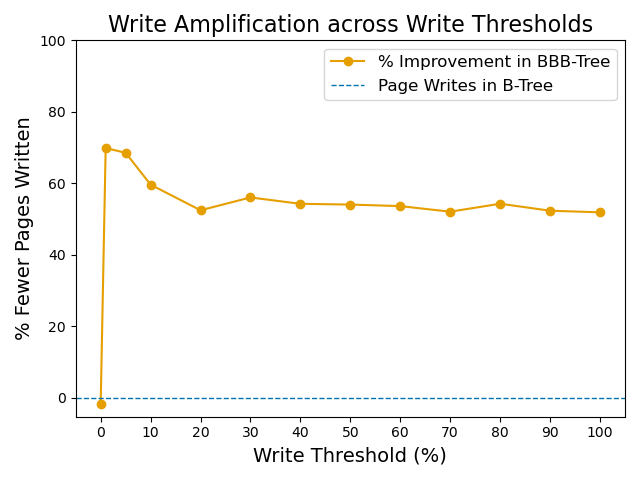
\includegraphics[width=0.6\textwidth]{figures/evaluation/pageviews_write_thresholds_improvement.png}
  \caption{The impact of different write thresholds on the amount of page writes per index with a 4 KB page size and 500 pages in the buffer pool. At 0\% threshold, we write every B-Tree node to disk after every change, leading to no improvement in write amplification. With higher thresholds, we can accumulate changes before writing them to disk, leading to significantly fewer page writes.}
  \label{fig:write_thresholds_improvement}
\end{figure}

\inlinesection{Without Buffering.}
With a write threshold of 0\%, we write every changed page to disk immediately, just as a traditional B-Tree would.
We can see a few more page writes with the BBB-Tree even, because we have a slightly smaller fanout due to the additional space required for tracking changes.
We will analyze the space overhead of the BBB-Tree in more detail below (see \autoref{sec:space_overhead}).

\inlinesection{With Buffering.}
Starting from a write threshold of 1\%, we can accumulate changes in the Delta Tree and reduce page writes significantly.
In fact, 1\% is the most significant step in reducing page writes of \textasciitilde70\% compared to the B-Tree.
With higher write thresholds, we accumulate more changes in the Delta Tree before writing them to disk, however the improvements become smaller.
There are three reasons for the diminishing return with increasing write thresholds:
\begin{enumerate}
\item \textbf{Fewer Changes Fit into a Page:} 
We achieve our goal of reducing page writes when we can accumulate changes on $y$ pages into a single page of the Delta Tree, where $y > 1$.
We can then save up to $y - 1$ page writes.
However, with larger write thresholds, fewer pages' changes fit into a single page.
For example, with a 1\% threshold, we can fit 100 page's changes into a single 4 KB page, while with a 25\% threshold, we can only fit 4 page's changes in the worst case.
The maximum accumulation factor $y$ decreases with larger write thresholds, leading to fewer potential savings in page writes.
\item \textbf{Less Likelihood to Batch Changes:}
With fewer changes fitting into a single page, the likelihood of batching changes in between Delta Tree page writes decreases.
For example, assume a Delta Tree node $d$ that holds $x$ delta arrays for $x$ B-Tree nodes.
This means, at some point $x$ B-Tree nodes have been modified. 
However, this does not directly translate to $x$ saved page writes, because $d$ itself might have been written to disk before all $x$ B-Tree nodes were modified.
Therefore, we only batch changes that happen between two writes of $d$.
When $d$ holds the changes of 100 B-Tree nodes, the likelihood of batching changes is much higher than when $d$ only holds the changes of 4 B-Tree nodes.
On average, we can save $\frac{y - 1}{s}$ page writes per Delta Node $d$, where $s$ is the number of times $d$ has been written to disk.
\item \textbf{More Leaf Nodes in Delta Tree:}
Additionally, with larger deltas, we require more leaf nodes in the Delta Tree to address all changes.
This introduces more page overhead in the system, leading to more page writes.
(The fanout itself is not affected, since inner nodes only hold fixed size \ac{PID}s as keys. The variable-sized deltas are only stored in the leaf nodes, so more pages need to be addressed by the Delta Tree.)
\end{enumerate}

\inlinesection{Stagnating Improvements.}
For all three reasons, we should see smaller improvements, the larger the write threshold becomes.
However, the improvements we see more or less stagnate after a write threshold of 20\%.
The reason is that we do not see many pages that are modified more than 20\% between page writes.
In \autoref{tab:modification-degree}, we can see the distribution of the modification degree for all modified B-Tree nodes at the time of eviction.
There are two reasons why we only see a small degree of change for most pages:

\begin{enumerate}
\item \textbf{Zipf-like Distribution:}
Due to the Zipf-like distribution of the keys in the workload, a small number of very popular articles receive a large number of operations, while the majority of articles receive only a few.
With an update ratio of 5\% of all operations in the workload, most articles are not updated at all (\textasciitilde 90\%).
Naturally, with updates scattered across the index, most pages are only slightly modified between page writes.
\item \textbf{Pages are Written Before They are Reach the Write Threshold:}
However, with a write threshold of 100\%, we should never write a B-Tree page to disk for the full workload (unless its new or it reaches a modification degree over 100\%).
We would expect at least some pages to be modified more than 20\% within the workload.
As shown in \autoref{tab:modification-degree}, all pages are modified by at most 30\% between evictions for a workload with 5\% updates.
To investigate this further, we looked at the same benchmark with a 100\% update ratio, i.e., all operations in the workload are updates.
This means that every article in the dataset is updated sooner or later in the workload.
Even with this extreme workload, we see that all pages are modified by at most 40\%.
The reason is that within the BBB-Tree we sometimes have to write B-Tree nodes instead of buffering their changes, even though its degree of chance is below the write threshold.
For example, when a page is new we force the page to disk at eviction.
More importantly though, we also do this when the Delta Tree is currently locked.
For example, when the Delta Tree receives a new root, we need to find space for the new node in the buffer manager.
If the buffer is full, we have to evict a page to free space in memory.
If we evict a B-Tree node that has been modified, we cannot buffer its changes in the Delta Tree, as it is currently locked.
Therefore, we have to write the B-Tree node to disk, even though its degree of change is below the write threshold.
This happens quite frequently in our benchmarks, and we observed that every B-Tree node is forced to be written at least once due to Delta Tree locks.
As a result, we never reach high degrees of change for any page, as we write them to disk before they can accumulate more changes.
Since smaller degrees of change are more attractive for our method for the reasons listed before, we do not investigate achieving higher write thresholds further.
\end{enumerate}

\inlinesection{Summary.}
Our method performs best with small write thresholds.
The sweet spot for the write threshold is between 1\% and 5\%, where we can achieve significant reductions in page writes without introducing too much space overhead in the Delta Tree.
We continue with a write threshold of 5\% in the following experiments, as it provides a good balance between write amplification reduction and space overhead.

\begin{table}[ht]
  \centering
    \begin{tabular}{l|cc}
    \toprule
    & \multicolumn{2}{c}{\textbf{Num. Pages}} \\
    \cmidrule(lr){2-3}
    \textbf{Modified} & \textbf{5\% Updates} & \textbf{100\% Updates} \\
    \midrule
    0--10\%   & 5274 &  38530\\
    10--20\%  & 670 & 1906\\
    20--30\%  & 1 & 61 \\
    30--40\%  & 0 & 1 \\
    $>$40\%  & 0 & 0 \\
    \bottomrule
  \end{tabular}
  \caption{Distribution and total count of pages by degree of change (percentage intervals). The grouped columns show the page counts for different update ratios in the workload. We see that most pages are only slightly modified between page writes.}
  \label{tab:modification-degree}
\end{table}

We only update a fraction (\textasciitilde10\%) of all entries in the dataset and many updates are to the same entry due to the Zipf-like distribution.
Therefore, most pages that are written to disk are modified only slightly, leading to a degree of change that is below the higher thresholds.
In fact, we could see in the benchmark metrics that the maximum degree of change for any page is 952 bytes, which is \textasciitilde23\% of a 4 KB page.
This means that with a write threshold of 23\% or higher, we already satiate the maximum degree of change for any page in the workload and therefore we cannot save any more page writes.
The small fluctuations we see in the results are due to the non-deterministic nature of the buffer pool management and page evictions.

To analyze the impact of write thresholds further, we will run the workload with different update ratios in the following section.

\subsection*{Impact of Update Ratios in Workload}
% More updates
% Only inserts
% Only lookups

\subsection*{Impact on Lookup Performance}

% TODO: Prettify the tables (axis labels, legends, captions, metrics, etc.)

\begin{table}[ht]
\centering
\caption{BM\_PageViews\_Insert\_DB}
\label{tab:bm_pageviews_insert_db}
\begin{tabular}{lrr}
\toprule
Metric & B-Tree & BBB-Tree \\
\midrule
Page Size [bytes] & 4096 & 4096 \\
Max. Pages in Buffer Pool & 100 & 100 \\
Write Threshold [\%] & 0 & 5 \\
\midrule
Real Time (ns) & 22021125.01 & 16292541.99 \\
CPU Time (ns) & 11619000 & 9610000 \\
\midrule
Number of Lookups (DB) & 0 & 0 \\
Number of Insertions (DB) & 11848 & 11848 \\
Number of Updates (DB) & 0 & 0 \\
\midrule
Number of Lookups (Index) & 0 & 474 \\
Number of Insertions (Index) & 11848 & 12049 \\
Number of Updates (Index) & 0 & 0 \\
Number of Deletions (Index) & 0 & 498 \\
\midrule
B-Tree Height & 2 & 2 \\
Delta Tree Height & 0 & 2 \\
Node Splits & 115 & 116 \\
\midrule
Bytes Written (Logically) & 189568 & 189568 \\
Bytes Written (Physically) & 2441216 & 1634304 \\
Write Amplification & 13 & 9 \\
\midrule
Buffer Accesses & 72007 & 73895 \\
Buffer Hits [\%] & 99 & 99 \\
Buffer Misses [\%] & 1 & 1 \\
\midrule
Num. Pages Created & 186 & 188 \\
Num. Slotted Pages Created & 70 & 70 \\
Num. Pages Evicted & 596 & 602 \\
Num. Pages Loaded & 507 & 509 \\
Num. Pages Write Deferred & 0 & 201 \\
Num. Pages Written & 596 & 399 \\
\bottomrule
\end{tabular}
\end{table}

\begin{table}[ht]
\centering
\caption{BM\_PageViews\_Lookup\_DB}
\label{tab:bm_pageviews_lookup_db}
\begin{tabular}{lrr}
\toprule
Metric & B-Tree & BBB-Tree \\
\midrule
Page Size [bytes] & 4096 & 4096 \\
Max. Pages in Buffer Pool & 100 & 100 \\
Write Threshold [\%] & 5 & 5 \\
\midrule
Real Time (ns) & 16211707.96 & 22320084.04 \\
CPU Time (ns) & 16187000 & 22229000 \\
\midrule
Number of Lookups (DB) & 29897 & 29897 \\
Number of Insertions (DB) & 0 & 0 \\
Number of Updates (DB) & 0 & 0 \\
\midrule
Number of Lookups (Index) & 29897 & 42811 \\
Number of Insertions (Index) & 0 & 0 \\
Number of Updates (Index) & 0 & 0 \\
Number of Deletions (Index) & 0 & 0 \\
\midrule
B-Tree Height & 2 & 2 \\
Delta Tree Height & 0 & 2 \\
Node Splits & 0 & 0 \\
\midrule
Bytes Written (Logically) & 0 & 0 \\
Bytes Written (Physically) & 0 & 0 \\
Write Amplification & 0 & 0 \\
\midrule
Buffer Accesses & 89692 & 115521 \\
Buffer Hits [\%] & 78 & 81 \\
Buffer Misses [\%] & 22 & 19 \\
\midrule
Num. Pages Created & 0 & 0 \\
Num. Slotted Pages Created & 0 & 0 \\
Num. Pages Evicted & 19603 & 21824 \\
Num. Pages Loaded & 19703 & 21924 \\
Num. Pages Write Deferred & 0 & 0 \\
Num. Pages Written & 0 & 0 \\
\bottomrule
\end{tabular}
\end{table}

\begin{table}[ht]
\centering
\caption{Comparison of BM\_PageViews\_Mixed\_DB and BM\_PageViews\_Mixed\_Index}
\label{tab:bm_pageviews_mixed_combined}
\begin{tabular}{l|rr|rr}
\toprule
Metric & \multicolumn{2}{c|}{BM\_PageViews\_Mixed\_DB} & \multicolumn{2}{c}{BM\_PageViews\_Mixed\_Index} \\
\cmidrule(lr){2-3} \cmidrule(lr){4-5}
 & B-Tree & BBB-Tree & B-Tree & BBB-Tree \\
\midrule
Page Size [bytes] & 4096 & 4096 & 4096 & 4096 \\
Max. Pages in Buffer Pool & 100 & 100 & 100 & 100 \\
Write Threshold [\%] & 5 & 5 & 5 & 5 \\
\midrule
Real Time (ns) & 70183334.00 & 73730334.00 & 30055833.98 & 16956374.98 \\
CPU Time (ns) & 39414000.00 & 47899000.00 & 14347000.00 & 13606000.00 \\
\midrule
Number of Lookups (DB) & 28394 & 28394 & 0 & 0 \\
Number of Insertions (DB) & 0 & 0 & 0 & 0 \\
Number of Updates (DB) & 1503 & 1503 & 0 & 0 \\
\midrule
Number of Lookups (Index) & 29897 & 43185 & 28394 & 33663 \\
Number of Insertions (Index) & 0 & 1334 & 0 & 1059 \\
Number of Updates (Index) & 1503 & 1503 & 1503 & 1503 \\
Number of Deletions (Index) & 0 & 1355 & 0 & 1076 \\
\midrule
B-Tree Height & 2 & 2 & 2 & 2 \\
Delta Tree Height & 0 & 2 & 0 & 2 \\
Node Splits & 0 & 6 & 0 & 7 \\
\midrule
Bytes Written (Logically) & 24048 & 24048 & 24048 & 24048 \\
Bytes Written (Physically) & 9719808 & 7417856 & 4136960 & 1241088 \\
Write Amplification & 404 & 308 & 172 & 52 \\
\midrule
Buffer Accesses & 92698 & 124701 & 59795 & 74660 \\
Buffer Hits [\%] & 79 & 82 & 94 & 92 \\
Buffer Misses [\%] & 21 & 18 & 6 & 8 \\
\midrule
Num. Pages Created & 0 & 6 & 0 & 7 \\
Num. Slotted Pages Created & 0 & 0 & 0 & 0 \\
Num. Pages Evicted & 19440 & 22962 & 3652 & 5589 \\
Num. Pages Loaded & 19540 & 23056 & 3752 & 5682 \\
Num. Pages Write Deferred & 0 & 1334 & 0 & 1059 \\
Num. Pages Written & 2373 & 1811 & 1010 & 303 \\
\bottomrule
\end{tabular}
\end{table}

\subsection*{Write Amplification (WIP)}

% uniform distribution of keys, random inserts
To compare the difference in write amplification between a B-Tree and a BBB-Tree, we create a database templated on each index and observe the number of page writes for different update set sizes.
We choose a page size of 4 KB as a default \cite{haas2023modern}, however we will be investigating the effect of different page sizes in the sensitivity analysis below.
We limit the size of the buffer pool to 100 pages.
We then benchmark the write amplification of each index when inserting a certain amount of tuples into the empty database.
The performance of the BBB-Tree is mainly determined by the number of inserts that we perform, as well as the \ac{WA} threshold (the threshold deciding whether a page is buffered in the Delta Tree or not).
In [TODO] we can see the benchmark for 10,000 tuples inserted across different \ac{WA} thresholds.
In [TODO], we can see the results for 100,000 tuples inserted.

For 10K tuples, we see a reduction in write amplification up to 28\% across all thresholds with our method.
For 100K tuples however, it depends on the \ac{WA} threshold.
We see a reduction in \ac{WA} for small thresholds (5-10\%) but an increase for larger thresholds (20-50\%).

Whenever we see an increase in \ac{WA} in this benchmark, it has a common factor: 
The number of nodes in the Delta Tree is large in relation to its base B-Tree.
For example, with 100K tuples inserted and a \ac{WA} threshold of 50\%, the Delta Tree was almost 1/3 of the B-Tree in size.
This is because Delta Arrays can become up to 50\% of a B-Tree node's size to mirror its changes.
If every B-Tree node was close to a 50\% change degree, each Delta Tree node could only hold up to two entries.
We require many nodes to address the changes.
However, a large Delta Tree is unfavourable. 
The larger the tree, the more likely it is that updates are scattered across the nodes, introducing write amplification in the Delta Tree itself.
We lose the batching effect that we are aiming for.
We essentially amplify the write amplification of the B-Tree. 

The smaller the threshold is, the smaller are the delta arrays per page.
Small delta arrays are favourable, since it keeps our Delta Tree small. 
The smaller the Delta Tree, the more we can benefit from a batching effect in that tree.

% Question 0: How much write amplification do we have in a traditional B-tree. How much in our approach? Show the bytes inserted by the user, the bytes written to the tree, the bytes written to storage.
% Question 1: Does the approach reduce write amplification compared to a traditional B-Tree?

% For 10K tuples we always saw a reduction in write amplification, for 100K tuples we saw an increase in write amplification.
% This is because we erase a lot of entries in the Delta Tree, which causes a lot of fragmentation and caused significantly more nodes.
% The higher the fanout of the tree, the higher the write amplification we introduce in the Delta Tree itself.
% We essentially amplified the write amplification in the system by introducing even more fanout in the Delta Tree.
% If the Delta Tree becomes to big in relation to the Base Tree, we do not have a reduction in write amplification anymore.
% When we compacitified after every erase, we saw a reduction in write amplification again.
% Now we reduce write amplification for small threshold (5-10%), but increase it for higher thresholds (20-50%).


% Write Amplification vs. Data size
% Write Amplification vs. Workload type (read-heavy, write-heavy, mixed)
% Number of writes to storage vs. workload type
% Average IO operations per update (baseline vs. our approach)

% \subsection*{Latency and Throughput}
% Latency vs. Workload type
% Throughput vs. Workload type
% Latency vs. Data size
% Throughput vs. Data size

\subsection*{Space Utilization and Memory Overhead}
\label{sec:space_overhead}
% Space Utilization vs. Data size (probably need more pages for fewer entries because slot size increases with delta tracking)
% Do we have more nodes in the system with tracking when reading only?

% When benchmarking with a buffer manager that can fit whole B-Tree, we see that we require one more node to address the same amount of entries.
% This is because we have to reserve space for delta tracking.
% Actually, this could also be the single node from the Delta Tree.

% When benchmarking with a WA-Threshold of 0%, we see that we require more nodes in the system. One for the empty delta tree but the rest is because we have need more nodes with delta tracking.

\subsection*{Variable Size Entries}

\subsection*{Sensitivity Analysis}
% WA vs Key Size
% WA vs Page Size
% WA vs Buffer Size
% WA vs Delta Size

\section{Discussion}
% “Our approach reduces write amplification by 40–60% while maintaining within 5% of baseline read latency.”11,848